
% This LaTeX was auto-generated from an M-file by MATLAB.
% To make changes, update the M-file and republish this document.

\documentclass{article}
\usepackage{graphicx}
\usepackage{color}
\usepackage{listings}
\usepackage[framed]{mcode}
\usepackage{fullpage}
\usepackage{amsmath}
\usepackage[utf8x]{inputenc}
\usepackage{import}
\usepackage{setspace}
\usepackage{hyperref}
\definecolor{lightgray}{gray}{0.5}
\setlength{\parindent}{0pt}

\begin{document}

    
    
%\section*{}


\title{BE 521: Homework 7 \\{\normalsize p300 Speller} \\{\normalsize Spring 2021}}
\author{34 points}
\date{Due: 3/23/2021 10 PM}
\maketitle \textbf{Objective:} Spell letters using neurosignals


\begin{center} \author{NAME HERE \\
  \normalsize Collaborators: COLLABORATORS HERE \\}
\end{center}


\subsection*{P300 Speller}
In this homework, you will work with data from a P300-based brain computer interface called BCI2000 (Schalk et al. 2004) that allows people to spell words by focusing their attention on a particular letter displayed on the screen. In each trial the user focused on a letter, and when that letter's row or column is flashed, the user's brain elicits a P300 evoked response. By analyzing whether a P300 signal was produced, across the flashes of many different rows or columns, the computer can determine the letter that the person is focusing on.


Figure 1 shows the letter matrix from one trial of this task.
\begin{figure}
 \centering
 \includegraphics[width=0.3\textwidth]{letterMat}
 \caption{The letter matrix for the P300 speller with the third row illuminated.
          If the user were focusing on any of the letters in the third row (M, N, O, P, Q, or R),
          their brain would emit a P300 response. Otherwise it would not.}
\end{figure}


\subsection*{Data Organization}
The data for this homework is stored in \verb|I521_A0008_D001| on the IEEG Portal.
The EEG in this dataset were recorded during 85 intended letter spellings. For each letter spelling, 12 row/columns were flashed 15 times in random order ($12 \times 15 = 180$ iterations). The EEG was recorded with a sampling rate of 240 Hz on a 64-channel scalp EEG.\\


The annotations for this dataset are organized in two layers as follows:
\begin{itemize}
    \item \verb|TargetLetter| annotation layer indicates the target
    letter (annotation.description) on which the user was focusing
    during the recorded EEG segment
    (annotation.start/annotation.stop). This layer is also provided
    as TargetLetterAnnots.mat.
    \item \verb|Stim| annotation layer indicates the row/column that
    is being flashed (annotation.description) and whether the target
    letter is contained in that flash (annotation.type). The
    recorded EEG during that flash is
    (annotation.start/annotation.stop). Note that this annotation
    layer is provided as StimAnnots.mat. It is NOT on the portal.
\end{itemize}
Hints: There are many annotations in this dataset and getting them all may take ~5-10 minutes. Once you retrieve the annotations once, save them for faster loading in the future. Also, use $\verb|{ }|$ to gather variables across structs for easier manipulation (e.g. $\verb|strcmp({annotations.type},'1')|$) \\

\begin{lstlisting}
clc; close all; clear;

cd('/Users/sppatankar/Developer/BE-521')
addpath(genpath('Homework_7'));
addpath(genpath('ieeg-matlab-1.14.49'))

session = IEEGSession('I521_A0008_D001', 'spatank', 'spa_ieeglogin.bin');
sampling_rate =  session.data.sampleRate;
num_channels = length(session.data.rawChannels);

load('TargetLetterAnnots.mat')
load('StimAnnots.mat')

% channel_data(num_channels) = struct();
% % divide start and stop by 1e6 to convert to s before pulling signal
%
% for channel = 1:num_channels
%     fprintf('Channel %d\n', channel);
%     channel_end_time = ...
%         session.data.rawChannels(channel).get_tsdetails.getEndTime/1e6; % s
%     fprintf('Loading channel %d.\n', channel);
%     channel_data(channel).signal = ...
%         session.data.getvalues(1:ceil(channel_end_time * sampling_rate), channel);
%     fprintf('Loaded channel %d.\n', channel);
%     on_target = [];
%     off_target = [];
%     for stim_idx = 1:length(Stim)
%         start_time = Stim(stim_idx).start/1e6; % s
%         start_idx = ceil(start_time * sampling_rate);
%         end_time = Stim(stim_idx).stop/1e6; % s
%         end_idx = ceil(end_time * sampling_rate);
%         window = channel_data(channel).signal(start_idx:end_idx)';
%         if strcmp(Stim(stim_idx).type, '1') % on target
%             on_target = [on_target; window];
%         else % off target
%             off_target = [off_target; window];
%         end
%     end
%     channel_data(channel).on_target = on_target;
%     channel_data(channel).off_target = off_target;
% end

load('Data/channel_data.mat');
\end{lstlisting}

\color{lightgray} \begin{lstlisting}IEEGSETUP: Adding 'ieeg-matlab.jar' to dynamic classpath
IEEGSETUP: Found log4j on Java classpath.
URL: https://www.ieeg.org/services
Client user: spatank
Client password: ****
\end{lstlisting} \color{black}

\begin{figure}
 \centering
 \includegraphics[width=0.3\textwidth]{letterMatInds}
 \caption{The row/column indices of the letter matrix, as encoded in the \textbf{Stim} annotation layer (annotation.description) matrix.}
\end{figure}


\subsection*{Topographic EEG Maps}
You can make topographic plots using the provided \verb|topoplotEEG| function. This function needs an ``electrode file.'' and can be called like
\begin{lstlisting}
 topoplotEEG(data,'eloc64.txt','gridscale',150)
\end{lstlisting}
where \verb|data| is the value to plot for each channel. This function plots the electrodes according to the map in Figure 3.
\begin{figure}
 \centering
 \includegraphics[width=\textwidth]{scalpEEGChans}
 \caption{The scalp EEG 64-channel layout.}
\end{figure}


\pagebreak
\section{Exploring the data}
In this section you will explore some basic properties of the data in \verb|I521_A0008_D001|.


\begin{enumerate}


 \item For channel 11 (Cz), plot the mean EEG for the target and non-target stimuli separately, (i.e. rows/columns including and not-including the desired character, respectively), on the same set of axes. Label your x-axis in milliseconds. (3 pts)

[ANSWER HERE]
\begin{lstlisting}
channel_11_on_target = mean(channel_data(11).on_target);
channel_11_off_target = mean(channel_data(11).off_target);
time = ((1:length(channel_11_on_target))/sampling_rate) * 1000; % ms

figure;
hold on
plot(time, channel_11_on_target, 'b', 'LineWidth', 1)
plot(time, channel_11_off_target, 'r', 'LineWidth', 1)
legend('On Target', 'Off Target', 'Location', 'NorthEast');
hold off
xlabel('Time (ms)');
ylabel('\muV');
title('Mean EEG Signal: Channel 11');
\end{lstlisting}


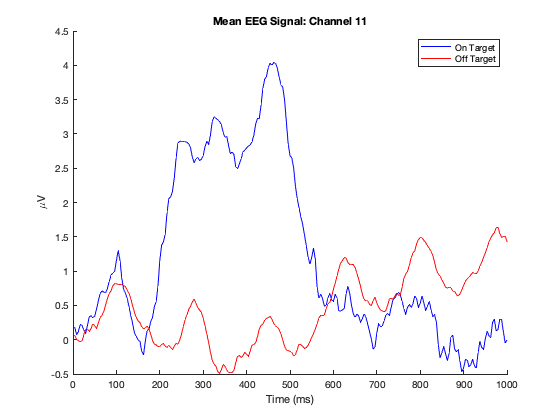
\includegraphics [width=5in]{spatank_hw7_01.png}

 \item Repeat the previous questions for channel 42 (T8). (1 pts)

[ANSWER HERE]
\begin{lstlisting}
channel_42_on_target = mean(channel_data(42).on_target);
channel_42_off_target = mean(channel_data(42).off_target);
time = ((1:length(channel_42_on_target))/sampling_rate) * 1000; % ms

figure;
hold on
plot(time, channel_42_on_target, 'b', 'LineWidth', 1)
plot(time, channel_42_off_target, 'r', 'LineWidth', 1)
legend('On Target', 'Off Target', 'Location', 'NorthEast');
hold off
xlabel('Time (ms)');
ylabel('\muV');
title('Mean EEG Signal: Channel 42');
\end{lstlisting}


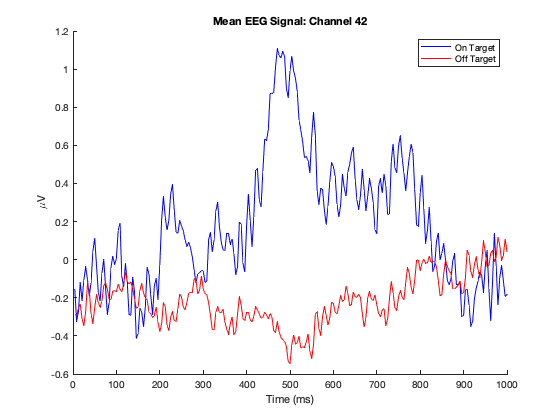
\includegraphics [width=5in]{spatank_hw7_02.png}

 \item Which of the two previous channels looks best for distinguishing between target and non-target stimuli? Which time points look best? Explain in a few sentences. (2 pts)

[ANSWER HERE]
\begin{lstlisting}
% Channel 11 looks better than channel 42 for distinguishing between target
% and non-target stimuli. The P300 response is less noisy and has a
% significantly higher voltage magnitude. The best time points in the
% signal for channel 11 are roughly between 200 and 600 ms.
\end{lstlisting}

 \item Compute the mean difference between the target and non-target stimuli for each channel at timepoint 300 ms averaged across all row/column flashes. Visualize these values using the \verb|topoplotEEG| function. Include a colorbar. (3 pts)

[ANSWER HERE]
\begin{lstlisting}
idx_300 = 300/1000 * sampling_rate;
diff_300 = zeros(1, num_channels);

for channel = 1:num_channels
    on_target_300 = mean(channel_data(channel).on_target(:, idx_300));
    off_target_300 = mean(channel_data(channel).off_target(:, idx_300));
    diff_300(channel) = on_target_300 - off_target_300;
end

figure;
topoplotEEG(diff_300, 'eloc64.txt', 'gridscale', 150)
\end{lstlisting}


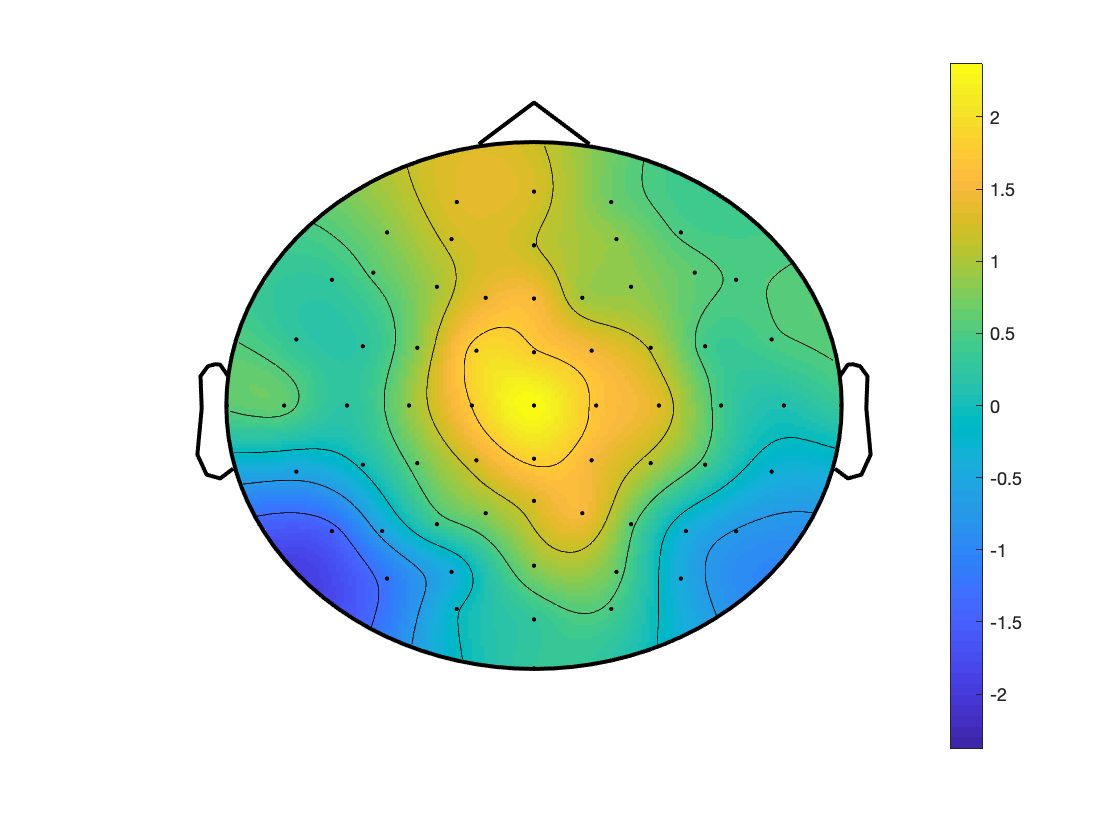
\includegraphics [width=5in]{spatank_hw7_03.png}

 \item How do the red and blue parts of this plot correspond to the plots from above? (2 pts)

[ANSWER HERE]
\begin{lstlisting}
% The greatest difference between on-target and off-target stimuli is
% observed for a number of channels near the center line near the top of
% the skull. Channel 11 is the most central of these channels and has the
% greatest difference. Channel 42 on the other hand is much further off the
% center and has a relatively low difference between the on-target and
% off-target stimuli signals at 300 ms. The figures above also support this
% as evidenced by the much lower magnitude of the signal for channel 42
% compared to that for channel 11.
\end{lstlisting}

\end{enumerate}
\section{Using Individual P300s in Prediction}
Hopefully the Question 1.4 convinced you that the Cz channel is a reasonably good channel to use in separating target from non-target stimuli in the P300. For the rest of the homework, you will work exclusively with this channel.
\begin{enumerate}
 \item Explain a potential advantage to using just one channel other than the obvious speed of calculation advantage. Explain one disadvantage. (3 pts)

[ANSWER HERE]
\begin{lstlisting}
% Somewhat counter to intuition, I think that using just one channel reduces
% the noise in the data. Since the P300 response may be measured over a
% wide range of time points, using all the channels can have an effect of
% increasing the overall signal magnitude while simultaneously causing any
% P300 spike to become less sharply distinguishable by pushing it into the
% background. A disadvantage of using just one channel's signal is that there
% are fewer features to use in a learning algorithm. For instance, the
% signal in two channels may deterministically help identify a target
% letter whereas either channel on its own may not.
\end{lstlisting}

 \item One simple way of identifying a P300 in a single trial (which we'll call the \emph{p300 score}) is to take the mean EEG from 250 to 450 ms and then subtract from it the mean EEG from 600 to 800 ms. What is the 	\emph{p300 score} for epoch (letter) 10, iteration 11 at electrode Cz? (3 pts)

[ANSWER HERE]
\begin{lstlisting}
channel = 11; % electrode Cz

epoch_number = 10;
epoch_data = TargetLetter(epoch_number);
all_epoch_trials = Stim((1:(12 * 15)) + (epoch_number - 1) * (12 * 15));

trial_number = 11;
start_time = all_epoch_trials(trial_number).start/1e6; % s
start_idx = ceil(start_time * sampling_rate);
end_time = all_epoch_trials(trial_number).stop/1e6; % s
end_idx = ceil(end_time * sampling_rate);
trial_signal = channel_data(channel).signal(start_idx:end_idx)';

window_1 = mean(trial_signal(250/1000 * sampling_rate : 450/1000 * sampling_rate));
window_2 = mean(trial_signal(600/1000 * sampling_rate : 800/1000 * sampling_rate));
p300_score = window_1 - window_2

% figure;
% plot(time, trial_signal, 'b', 'LineWidth', 1)
% xlabel('Time (ms)');
% ylabel('\muV');
% title('EEG Signal: Channel 11, Epoch 10, Trial 11');
\end{lstlisting}

\color{lightgray} \begin{lstlisting}
p300_score =

    0.6554

\end{lstlisting} \color{black}

 \item Plot the \emph{p300 scores} for each row/column in epoch 27 at electrode Cz. (3 pts)

[ANSWER HERE]
\begin{lstlisting}
lookup = ['ABCDEF';'GHIJKL';'MNOPQR';'STUVWX';'YZ1234';'56789_'];

epoch_number = 27;
epoch_data = TargetLetter(epoch_number);
all_epoch_trials = Stim((1:(12 * 15)) + (epoch_number - 1) * (12 * 15));

p300_scores_mat = NaN(12, 15); % lots of redundant memory allocation!

row_col_counters = ones(1, 12);

for trial_number = 1:length(all_epoch_trials)
    start_time = all_epoch_trials(trial_number).start/1e6; % s
    start_idx = ceil(start_time * sampling_rate);
    end_time = all_epoch_trials(trial_number).stop/1e6; % s
    end_idx = ceil(end_time * sampling_rate);
    trial_signal = channel_data(channel).signal(start_idx:end_idx)';
    window_1 = mean(trial_signal(250/1000 * sampling_rate : 450/1000 * sampling_rate));
    window_2 = mean(trial_signal(600/1000 * sampling_rate : 800/1000 * sampling_rate));
    switch all_epoch_trials(trial_number).description
    case '1'
        p300_scores_mat(1, row_col_counters(1)) = window_1 - window_2;
        row_col_counters(1) = row_col_counters(1) + 1;
    case '2'
        p300_scores_mat(2, row_col_counters(2)) = window_1 - window_2;
        row_col_counters(2) = row_col_counters(2) + 1;
    case '3'
        p300_scores_mat(3, row_col_counters(3)) = window_1 - window_2;
        row_col_counters(3) = row_col_counters(3) + 1;
    case '4'
        p300_scores_mat(4, row_col_counters(4)) = window_1 - window_2;
        row_col_counters(4) = row_col_counters(4) + 1;
    case '5'
        p300_scores_mat(5, row_col_counters(5)) = window_1 - window_2;
        row_col_counters(5) = row_col_counters(5) + 1;
    case '6'
        p300_scores_mat(6, row_col_counters(6)) = window_1 - window_2;
        row_col_counters(6) = row_col_counters(6) + 1;
    case '7'
        p300_scores_mat(7, row_col_counters(7)) = window_1 - window_2;
        row_col_counters(7) = row_col_counters(7) + 1;
    case '8'
        p300_scores_mat(8, row_col_counters(8)) = window_1 - window_2;
        row_col_counters(8) = row_col_counters(8) + 1;
    case '9'
        p300_scores_mat(9, row_col_counters(9)) = window_1 - window_2;
        row_col_counters(9) = row_col_counters(9) + 1;
    case '10'
        p300_scores_mat(10, row_col_counters(10)) = window_1 - window_2;
        row_col_counters(10) = row_col_counters(10) + 1;
    case '11'
        p300_scores_mat(11, row_col_counters(11)) = window_1 - window_2;
        row_col_counters(11) = row_col_counters(11) + 1;
    case '12'
        p300_scores_mat(12, row_col_counters(12)) = window_1 - window_2;
        row_col_counters(12) = row_col_counters(12) + 1;
    end
end

cols = p300_scores_mat(1:6, :);
rows = p300_scores_mat(7:12, :);
[~, row_idx] = max(mean(rows, 2, 'omitnan'));
[~, col_idx] = max(mean(cols, 2, 'omitnan'));

figure;
subplot(2, 1, 1);
boxplot(rows')
title('Select Target: Epoch 27', 'FontSize', 15);
xlabel('Row ID', 'FontSize', 15);
subplot(2, 1, 2);
boxplot(cols')
xlabel('Column ID', 'FontSize', 15);


label = epoch_data.description
prediction = lookup(row_idx, col_idx)
\end{lstlisting}

\color{lightgray} \begin{lstlisting}
label =

    'B'


prediction =

    'B'

\end{lstlisting} \color{black}


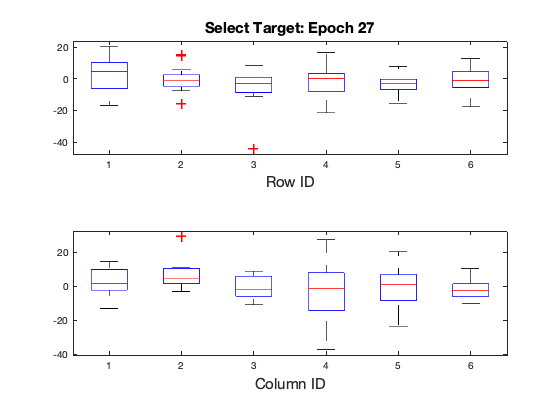
\includegraphics [width=5in]{spatank_hw7_04.png}

 \item Based on your previous answer for epoch 27, what letter do you predict the person saw? Is this prediction correct? (2 pts)

\begin{lstlisting}
% The predicted letter ('B') matches the target letter ('B').
\end{lstlisting}
[ANSWER HERE]

 \item Using this \emph{p300 score}, predict (and print out) the letter viewed at every epoch. What was you prediction accuracy? (2 pts)

[ANSWER HERE]
\begin{lstlisting}
correct = 0;

for epoch_number = 1:length(TargetLetter)
    epoch_data = TargetLetter(epoch_number);
    all_epoch_trials = Stim((1:(12 * 15)) + (epoch_number - 1) * (12 * 15));
    p300_scores_mat = NaN(12, 15);
    row_col_counters = ones(1, 12);
    for trial_number = 1:length(all_epoch_trials)
        start_time = all_epoch_trials(trial_number).start/1e6; % s
        start_idx = ceil(start_time * sampling_rate);
        end_time = all_epoch_trials(trial_number).stop/1e6; % s
        end_idx = ceil(end_time * sampling_rate);
        trial_signal = channel_data(channel).signal(start_idx:end_idx)';
        window_1 = mean(trial_signal(250/1000 * sampling_rate : 450/1000 * sampling_rate));
        window_2 = mean(trial_signal(600/1000 * sampling_rate : 800/1000 * sampling_rate));
        switch all_epoch_trials(trial_number).description
        case '1'
            p300_scores_mat(1, row_col_counters(1)) = window_1 - window_2;
            row_col_counters(1) = row_col_counters(1) + 1;
        case '2'
            p300_scores_mat(2, row_col_counters(2)) = window_1 - window_2;
            row_col_counters(2) = row_col_counters(2) + 1;
        case '3'
            p300_scores_mat(3, row_col_counters(3)) = window_1 - window_2;
            row_col_counters(3) = row_col_counters(3) + 1;
        case '4'
            p300_scores_mat(4, row_col_counters(4)) = window_1 - window_2;
            row_col_counters(4) = row_col_counters(4) + 1;
        case '5'
            p300_scores_mat(5, row_col_counters(5)) = window_1 - window_2;
            row_col_counters(5) = row_col_counters(5) + 1;
        case '6'
            p300_scores_mat(6, row_col_counters(6)) = window_1 - window_2;
            row_col_counters(6) = row_col_counters(6) + 1;
        case '7'
            p300_scores_mat(7, row_col_counters(7)) = window_1 - window_2;
            row_col_counters(7) = row_col_counters(7) + 1;
        case '8'
            p300_scores_mat(8, row_col_counters(8)) = window_1 - window_2;
            row_col_counters(8) = row_col_counters(8) + 1;
        case '9'
            p300_scores_mat(9, row_col_counters(9)) = window_1 - window_2;
            row_col_counters(9) = row_col_counters(9) + 1;
        case '10'
            p300_scores_mat(10, row_col_counters(10)) = window_1 - window_2;
            row_col_counters(10) = row_col_counters(10) + 1;
        case '11'
            p300_scores_mat(11, row_col_counters(11)) = window_1 - window_2;
            row_col_counters(11) = row_col_counters(11) + 1;
        case '12'
            p300_scores_mat(12, row_col_counters(12)) = window_1 - window_2;
            row_col_counters(12) = row_col_counters(12) + 1;
        end
    end
    cols = p300_scores_mat(1:6, :);
    rows = p300_scores_mat(7:12, :);
    [~, row_idx] = max(mean(rows, 2, 'omitnan'));
    [~, col_idx] = max(mean(cols, 2, 'omitnan'));
    label = epoch_data.description;
    prediction = lookup(row_idx, col_idx);
    if strcmp(label, prediction)
        correct = correct + 1;
    end
    fprintf('Label: %c, Prediction: %c\n', label, prediction);
end

prediction_accuracy = (correct/length(TargetLetter)) * 100

% This prediction accuracy is significantly better than when predictions
% are made at random (1/36 = 2.8%).
\end{lstlisting}

\color{lightgray} \begin{lstlisting}Label: E, Prediction: 4
Label: A, Prediction: A
Label: E, Prediction: 8
Label: V, Prediction: V
Label: Q, Prediction: E
Label: T, Prediction: U
Label: D, Prediction: F
Label: O, Prediction: O
Label: J, Prediction: 8
Label: G, Prediction: I
Label: 8, Prediction: O
Label: R, Prediction: W
Label: B, Prediction: B
Label: R, Prediction: M
Label: G, Prediction: J
Label: O, Prediction: O
Label: N, Prediction: F
Label: C, Prediction: C
Label: E, Prediction: F
Label: D, Prediction: D
Label: H, Prediction: 9
Label: C, Prediction: C
Label: T, Prediction: T
Label: U, Prediction: X
Label: I, Prediction: I
Label: D, Prediction: D
Label: B, Prediction: B
Label: P, Prediction: 6
Label: U, Prediction: U
Label: H, Prediction: 1
Label: M, Prediction: A
Label: E, Prediction: W
Label: M, Prediction: R
Label: 6, Prediction: 5
Label: O, Prediction: I
Label: U, Prediction: O
Label: X, Prediction: K
Label: O, Prediction: O
Label: C, Prediction: I
Label: F, Prediction: Q
Label: O, Prediction: O
Label: U, Prediction: O
Label: K, Prediction: C
Label: W, Prediction: X
Label: A, Prediction: E
Label: 4, Prediction: _
Label: V, Prediction: T
Label: J, Prediction: G
Label: E, Prediction: K
Label: F, Prediction: 4
Label: R, Prediction: R
Label: Z, Prediction: 2
Label: R, Prediction: 3
Label: O, Prediction: G
Label: L, Prediction: L
Label: H, Prediction: H
Label: Y, Prediction: Y
Label: N, Prediction: 6
Label: Q, Prediction: Q
Label: D, Prediction: _
Label: W, Prediction: K
Label: _, Prediction: X
Label: E, Prediction: E
Label: K, Prediction: 9
Label: T, Prediction: V
Label: L, Prediction: L
Label: B, Prediction: R
Label: W, Prediction: X
Label: X, Prediction: T
Label: E, Prediction: K
Label: P, Prediction: K
Label: O, Prediction: P
Label: U, Prediction: I
Label: I, Prediction: H
Label: K, Prediction: N
Label: Z, Prediction: G
Label: E, Prediction: F
Label: R, Prediction: 4
Label: Y, Prediction: L
Label: O, Prediction: L
Label: O, Prediction: U
Label: T, Prediction: S
Label: H, Prediction: B
Label: Q, Prediction: Q
Label: I, Prediction: R

prediction_accuracy =

   27.0588

\end{lstlisting} \color{black}

\end{enumerate}
\section{Automating the Learning}
In Section 2, you used a fairly manual method for predicting the letter. Here, you will have free rein to use put any and all learning techniques to try to improve your testing accuracy.
\begin{enumerate}
 \item Play around with some ideas for improving/generalizing the prediction paradigm used in the letter prediction. Use the first 50 letter epochs as the training set and the later 35 for validation. Here, you are welcome to hard-code in whatever parameters you like/determine to be optimal. What is the optimal validation accuracy you get? Note: don't worry too much about accuracy, we are more interested in your thought process. (4 pts)

[ANSWER HERE]
\begin{lstlisting}
num_features = 3;
LLFn = @(x) sum(abs(diff(x)));
areaFn = @(x) sum(abs(x));

num_training_points = 50 * 12 * 15;
train_feats = zeros(num_training_points, num_features);
train_labels = zeros(num_training_points, 1);
idx = 1;
for epoch_number = 1:50
    epoch_data = TargetLetter(epoch_number);
    stim_idx = (1:(12 * 15)) + (epoch_number - 1) * (12 * 15);
    all_epoch_trials = Stim(stim_idx);
    for trial_number = 1:length(all_epoch_trials)
        start_time = all_epoch_trials(trial_number).start/1e6; % s
        start_idx = ceil(start_time * sampling_rate);
        end_time = all_epoch_trials(trial_number).stop/1e6; % s
        end_idx = ceil(end_time * sampling_rate);
        trial_signal = channel_data(channel).signal(start_idx:end_idx)';
        window_1 = mean(trial_signal(250/1000 * sampling_rate : 450/1000 * sampling_rate));
        window_2 = mean(trial_signal(600/1000 * sampling_rate : 800/1000 * sampling_rate));
        train_feats(idx, 1) = window_1 - window_2;
        train_feats(idx, 2) = LLFn(trial_signal);
        train_feats(idx, 3) = areaFn(trial_signal);
        train_labels(idx) = ...
            str2double(all_epoch_trials(trial_number).type);
        idx = idx + 1;
    end
end

train_feats_norm = (train_feats - mean(train_feats))./std(train_feats);
Mdl = fitcsvm(train_feats_norm, train_labels, 'KernelFunction', 'rbf');
train_labels_pred = predict(Mdl, train_feats_norm);
train_accuracy = sum(train_labels == train_labels_pred)/length(train_labels)

num_val_points = 35 * 12 * 15;
val_feats = zeros(num_val_points, num_features);
val_labels = zeros(num_val_points, 1);
idx = 1;
for epoch_number = 51:length(TargetLetter)
    fprintf('Validation Epoch: %d\n', epoch_number);
    stim_idx = (1:(12 * 15)) + (epoch_number - 1) * (12 * 15);
    all_epoch_trials = Stim(stim_idx);
    for trial_number = 1:length(all_epoch_trials)
        start_time = all_epoch_trials(trial_number).start/1e6; % s
        start_idx = ceil(start_time * sampling_rate);
        end_time = all_epoch_trials(trial_number).stop/1e6; % s
        end_idx = ceil(end_time * sampling_rate);
        trial_signal = channel_data(channel).signal(start_idx:end_idx)';
        window_1 = mean(trial_signal(250/1000 * sampling_rate : 450/1000 * sampling_rate));
        window_2 = mean(trial_signal(600/1000 * sampling_rate : 800/1000 * sampling_rate));
        val_feats(idx, 1) = window_1 - window_2;
        val_feats(idx, 2) = LLFn(trial_signal);
        val_feats(idx, 3) = areaFn(trial_signal);
        val_labels(idx) = ...
            str2double(all_epoch_trials(trial_number).type);
        idx = idx + 1;
    end
end

val_feats_norm = (val_feats - mean(train_feats))./std(train_feats);
val_labels_pred = predict(Mdl, val_feats_norm);
val_accuracy = sum(val_labels == val_labels_pred)/length(val_labels)
\end{lstlisting}

\color{lightgray} \begin{lstlisting}
train_accuracy =

    0.8342

Validation Epoch: 51
Validation Epoch: 52
Validation Epoch: 53
Validation Epoch: 54
Validation Epoch: 55
Validation Epoch: 56
Validation Epoch: 57
Validation Epoch: 58
Validation Epoch: 59
Validation Epoch: 60
Validation Epoch: 61
Validation Epoch: 62
Validation Epoch: 63
Validation Epoch: 64
Validation Epoch: 65
Validation Epoch: 66
Validation Epoch: 67
Validation Epoch: 68
Validation Epoch: 69
Validation Epoch: 70
Validation Epoch: 71
Validation Epoch: 72
Validation Epoch: 73
Validation Epoch: 74
Validation Epoch: 75
Validation Epoch: 76
Validation Epoch: 77
Validation Epoch: 78
Validation Epoch: 79
Validation Epoch: 80
Validation Epoch: 81
Validation Epoch: 82
Validation Epoch: 83
Validation Epoch: 84
Validation Epoch: 85

val_accuracy =

    0.8333

\end{lstlisting} \color{black}

 \item Describe your algorithm in detail. Also describe what you tried that didn't work. (6 pts)

[ANSWER HERE]
\begin{lstlisting}
% In the first instance, I tried a simple binary SVM classifier to predict
% whether a given signal trace for a stimulation was a P300 or not. Having
% done this for all of the stimulations regardless of the target letter, I
% found that the training accuracy for an SVM with the RBF kernel is
% 83.42%. The validation accuracy is 83.3%. In all of my tests, I use three
% features when training the model: the P300 score, line length, and area.
% The training data is Z-scored before being passed to a model. With the
% binary classifier, I noticed that the model heavily
% leans towards predicting that every stimulation is not a P300. This is
% because the data contains a disproportionately high number of non-P300
% responses. Future work may try to randomly sample from the training data
% in a way that attempts to balance the frequencies of the two classes.

% For the main problem, which is to predict a letter given a stimulus
% response, one approach is to train separate classifiers for each character of
% interest in the target data. This involves separating the Stim
% annotations based on their corresponding target letter from the
% TargetLetter annotations. These 36 classifiers can be used to assign
% scores to each predicted letter, and the classifier with the largest
% score can be treated as the successful model.

% Another approach is to use the outputs of the binary classification as
% guides. For instance, for a given epoch, we can ask whether a P300
% response occurred using the binary classifier for each of the 180 trials
% that make up the epoch. For those trials where the binary classifier
% predicts a P300, we can seek the row/column that was displayed. At the
% end of the epoch, we will have collected a set of rows and columns that
% are predicted to have evoked a P300 response. We can predict the
% character corresponding to the most frequent row and most frequent column
% as the focus of the participant's attention. Unfortunately, when I
% attempted this strategy, my binary classifier decided that there were no
% P300 responses. As a result, I was not able to successfully assign target
% letters to epochs.
\end{lstlisting}

\end{enumerate}
\end{document}




\end{document}
    
